%%%%%%%%%%%%%%%%%%%%%%%%%%%%%%%%%%%%%%%%%%%%%%%%%%%%%%%%%%%%%%%%%%%%%%%%
% change some parameters to be inline with our intended visual identiy
% 
% Create HaitzmannM::03/02/2021
%
% in progress
%
% indicate major changes, inclusions with initials and date
% XX::DDMMYYYY
%%%%%%%%%%%%%%%%%%%%%%%%%%%%%%%%%%%%%%%%%%%%%%%%%%%%%%%%%%%%%%%%%%%%%%%%
%%%%%%%%%%%%%%%%%%%%%%%%%%%%
%additional packages
%%%%%%%%%%%%%%%%%%%%%%%%%%%%
\usepackage{booktabs}
\usepackage{xcolor} % for colour
%\usepackage{background}
\usepackage{booktabs}
\usepackage{longtable}
\usepackage{array}
\usepackage{multirow}
\usepackage{wrapfig}
\usepackage{float}
\usepackage{subfig}
\usepackage{colortbl}
\usepackage{pdflscape}
\usepackage{tabu}
\usepackage{threeparttable}
\usepackage{threeparttablex}
\usepackage[normalem]{ulem}
\usepackage{makecell}
\usepackage{xcolor}
\usepackage{animate}

\usepackage{fontawesome5}

%%%%%%%%%%%%%%%%%%%%%%%%%%%%
%visual id color logo chapter header
%%%%%%%%%%%%%%%%%%%%%%%%%%%%
\definecolor{unidoblue}{RGB}{0,156,220}
%\definecolor{unidosuppl}{RGB}{220, 64, 0} %#alternative Maroon hexadecimal color #800000 {128,0,0}
\definecolor{unidosuppl}{RGB}{128,0,0} %#alternative Maroon hexadecimal color #800000 {128,0,0}

\newsavebox{\unidologo}
\savebox{\unidologo}{
\includegraphics[]{img/Unido_EN_Light_Blue.png}}

\newsavebox{\unidologowhite}
\savebox{\unidologowhite}{
\includegraphics[]{img/Unido_EN_White.png}}

\newsavebox{\unidologoblack}
\savebox{\unidologoblack}{
\includegraphics[]{img/Unido_EN_Black.png}}

%horizontal blue line
\newcommand*{\HRule}{\color{unidoblue}\hrule width 1\textwidth height 2pt} % <===========================
%\newcommand{\HRule}{\color{unidoblue}\rule{\textwidth}{0.1mm}}

\usepackage{fontspec}
%\setmainfont{Calibri}
%\setmainfont[Path=/usr/share/fonts/truetype/calibri/,
%    BoldItalicFont=calibriz.ttf,
%    BoldFont      =calibrib.ttf,
%    ItalicFont    =calibrii.ttf]{calibri.ttf}

%\usepackage{FiraSans}
%%DOES NOT WORK, Meta Pro NOrm not recognized
% UNIDO Font family
\usepackage[abspath]{currfile}
\setmainfont[
  %Path=\currfileabsdir, 
  %Path=H:/WORK/QUEST/Analysis/YB-2021-addendum/meta-pro-cufonfonts/
  Path = ./meta-pro-cufonfonts/,
  Renderer=Basic, Ligatures={TeX},Scale=MatchUppercase,
  %UprightFont    = meta-pro-cufonfonts/FFMetaProCondRg.TTF,
  ItalicFont     = FFMetaProCondRgIt.TTF,
  BoldFont       = FFMetaProCondBd.TTF,
  BoldItalicFont = FFMetaProCondBdIt.TTF,
  SmallCapsFont  = FFMetaProCondRg.TTF,
  SmallCapsFeatures= {Letters=SmallCaps}
  ]{FFMetaProCondRg}
%\setmainfont[Path=C:/Users/marti/Documents/Arbeit/UNIDO/H/WORK/QUEST/Analysis/YB-2021-addendum/meta-pro-cufonfonts/]{FFMetaProCondRg.TTF}
%%%%
 %need for xelatex in combinaitn with tufte pdf
  % Set up the spacing using fontspec features
  \renewcommand\allcapsspacing[1]{{\addfontfeature{LetterSpace=15}#1}}
  \renewcommand\smallcapsspacing[1]{{\addfontfeature{LetterSpace=10}#1}}
%%MetaPro does not have own SmallCaps, so use uppercase
\renewcommand{\textsc}[1]{\smallcapsspacing{\textsmallcaps{#1}}}
\renewcommand{\smallcaps}[1]{\smallcapsspacing{\scshape\MakeTextUppercase{#1}}}

%change section heder format
% add numbers to chapters, sections, subsections
\setcounter{secnumdepth}{2}

% chapter format
\titleformat{\chapter}%
  {\huge\rmfamily\itshape\color{unidoblue}}% format applied to label+text
  {\llap{\colorbox{unidoblue}{\parbox{1.5cm}{\hfill\itshape\huge\color{white}\thechapter}}}}% label
  {2pt}% horizontal separation between label and title body
  {}% before the title body
  [\HRule]% after the title body

% section format
\titleformat{\section}%
  {\normalfont\Large\itshape\color{unidoblue}}% format applied to label+text
  {\llap{\colorbox{unidoblue}{\parbox{1.5cm}{\hfill\color{white}\thesection}}}}% label
  {1em}% horizontal separation between label and title body
  {}% before the title body
  [\HRule]% after the title body

% subsection format
\titleformat{\subsection}%
  {\normalfont\large\itshape\color{unidoblue}}% format applied to label+text
  {\llap{\colorbox{unidoblue}{\parbox{1.5cm}{\hfill\color{white}\thesubsection}}}}% label
  {1em}% horizontal separation between label and title body
  {}% before the title body
  [\HRule]% after the title body

%%%%%%%%%%%%%%%%%%%%%%%%%%%%
%ADAPT TITLEPAGE
%%%%%%%%%%%%%%%%%%%%%%%%%%%%

%%%% additional Picture on titlepage
\newsavebox{\titlepagepic}
\savebox{\titlepagepic}{
\includegraphics[width=\linewidth,height=0.3\paperheight]{img/imagetitlepage_maroon.pdf}}

%%%%Titlepagearea style logo and area
\usepackage{tikz}
\usetikzlibrary{calc,positioning}% [0]
\def\TitlePageAreaLogoLine{%
  %%%%Blue Line at top paperwidht
  \tikz [remember picture,overlay]%
    \draw [draw=white, fill={rgb,255:red,0; green,156; blue,220}]($(current page.south west)!0.9!(current page.north west)$) rectangle  ($(current page.south east)!0.895!(current page.north east)$);
  %%%%LOGO topleft corneer
  \tikz [remember picture,overlay]%
    \node [anchor=north west] (logo) at (-2cm,2.5cm) {\resizebox{!}{2cm}{\usebox{\unidologo}}};
 %%%%shaded area top
  \tikz [remember picture,overlay]%
    \shade [top color={rgb,255:red,0; green,156; blue,220},bottom color=white] ($(current page.south west)!0.89!(current page.north west)$) rectangle ($(current page.south east)!0.7!(current page.north east)$);   
 %%%%titlepic 
  \tikz [remember picture,overlay]%
    \node [anchor=south west] (titlepic) at ($(current page.south west)!0.08!(current page.north west)$) {\resizebox{\paperwidth}{!}{\usebox{\titlepagepic}}};
  %%%%bottom area 
  \tikz [remember picture,overlay]%
        \shade [bottom color={rgb,255:red,0; green,156; blue,220},top color=white]($(current page.south west)!0!(current page.north west)$) rectangle  ($(current page.south east)!0.1!(current page.north east)$);
%    \draw [draw={rgb,255:red,0; green,156; blue,220}, fill={rgb,255:red,0; green,156; blue,220}]($(current page.south west)!0!(current page.north west)$) rectangle  ($(current page.south east)!0.1!(current page.north east)$);
  %%%%bottom area text
  \tikz [remember picture,overlay]%
    \node at (current page.south) [%
        draw={rgb,255:red,0; green,156; blue,220},
        inner sep=14pt,
        fill={rgb,255:red,0; green,156; blue,220},
        fill opacity=0.01,
        text=white,
        text opacity = 1,
        draw opacity = 0.01,
        above=0.5cm,
        font=\sffamily\Large
    ] {INCLUSIVE AND SUSTAINABLE INDUSTRIAL DEVELOPMENT};

 }


%%%%%%%%%%%%%%%%%%%
%Book end page 
\usetikzlibrary{calc,positioning}% [0]
\def\TitlePageAreaPagePlus{%
%%%%logo 
  \tikz [remember picture,overlay]%
    \node [anchor=south west] (logo) at (-1cm, -23.5cm) {\resizebox{!}{2cm}{\usebox{\unidologoblack}}};
}


%%%%%%%%Adapt titlepage

\newcommand{\plainsubtitle}{}%     plain-text-only subtitle
\newcommand{\subtitle}[1]{%
  \gdef\@subtitle{#1}%
  \renewcommand{\plainsubtitle}{#1}% use provided plain-text title
  \ifthenelse{\isundefined{\hypersetup}}%
    {}% hyperref is not loaded; do nothing
    {\hypersetup{pdftitle={\plaintitle: \plainsubtitle{}}}}% set the PDF metadata title
}

\renewcommand{\maketitlepage}[0]{%

\cleardoublepage%
{%
\sffamily%
\TitlePageAreaLogoLine
%\noindent\makebox[\paperwidth]{\color{unidoblue}\rule{\paperwidth}{2pt}} 
%\resizebox{!}{2cm}{\usebox{\unidologo}}
%\vspace{0.1cm}
%\HRule  
\vspace{1cm}
  \begin{fullwidth}%
 \fontsize{16}{20}\selectfont\par\noindent\textcolor{darkgray}{\allcaps{\thanklessauthor}}%
  \vspace{5.5pc}%
  \fontsize{32}{40}\selectfont\par\noindent\textcolor{darkgray}{\allcaps{\thanklesstitle}}%
  \vspace{3pc}%
  \fontsize{20}{28}\selectfont\par\noindent\textcolor{darkgray}{\allcaps{\plainsubtitle}}%
  \vfill%
  \fontsize{14}{16}\selectfont\par\noindent\allcaps{\thanklesspublisher}%
  %\vspace{0.1pc}%
  %\noindent\resizebox{!}{9cm}{\usebox{\titlepagepic}}
\end{fullwidth}%

\thispagestyle{empty}%

%%%%%add empty page
\newpage\null\thispagestyle{empty}\newpage

%%%%%add a third titlepage
\TitlePageAreaPagePlus
\sffamily
  \begin{fullwidth}%
 \fontsize{16}{20}\selectfont\par\noindent\textcolor{darkgray}{\allcaps{\thanklessauthor}}%
  \vspace{5.5pc}%
  \fontsize{32}{40}\selectfont\par\noindent\textcolor{darkgray}{\allcaps{\thanklesstitle}}%
  \vspace{3pc}%
  \fontsize{20}{28}\selectfont\par\noindent\textcolor{darkgray}{\allcaps{\plainsubtitle}}%
\end{fullwidth}%
\thispagestyle{empty}
%%
\newpage
%%%%% add a page with Disclaimer:

\singlespacing
{\normalfont\Large\itshape\color{unidoblue}\paragraph{About this publication}\hspace*{\fill} \\
\normalfont\color{black}{
\begin{fullwidth}
The International Yearbook of Industrial Statistics published by UNIDO contains a wealth of information on the level, structure and growth of world manufacturing. Data are presented at the most detailed level of 155 manufacturing industries. While these data are used by researchers to carry out in-depth economic analyses of structural transformation, many users have requested more concise statistical information on overall growth trends and the structure of global manufacturing.

\noindent This publication serves as an addendum to the International Yearbook of Industrial Statistics 2021 and provides some important statistical information on global manufacturing. The publication is compiled from data published in the Yearbook and other data products of UNIDO Statistics.

\noindent The publication is compiled and disseminated by UNIDO Statistics.
\end{fullwidth}
}
}
\vspace{1pc}
{\normalfont\Large\itshape\color{unidoblue}\paragraph{Acknowledgements}\hspace*{\fill} \\
\normalfont\color{black}{
\begin{fullwidth}
Add here all necessary acknowledgements.
\end{fullwidth}
}
}
\vspace*{\fill}

%\paragraph{Disclaimer}\hspace*{\fill} \\
{\small\normalfont\color{black}{ 
%\begin{justify}
\begin{fullwidth}
Copyright \textcopyright 2021 United Nations Industrial Development Organization

\noindent The designations employed and the presentation of the material in this document do not imply the expression of any opinion whatsoever on the part of the Secretariat of the United Nations Industrial Development Organization (UNIDO) concerning the legal status of any country, territory, city or area or of its authorities, or concerning the delimitation of its frontiers or boundaries, or its economic system or degree of development.

\noindent Designations such as „developed“, „industrialized“ and „developing“ are intended for statistical convenience and do not necessarily express a judgment about the stage reached by a particular country or area in the development process. Mention of firm names or commercial products does not constitute an endorsement by UNIDO.

\noindent Material in this publication may be freely quoted or reprinted, but acknowledgement is requested, together with a copy of the publication containing the quotation or reprint.

\noindent For reference and citation, please use: United Nations Industrial Development Organization, 2021. TITLE.Vienna.
\end{fullwidth}
%\end{justify}
}}
}

\thispagestyle{empty}
\clearpage

}
%%%%%%%%
\pagenumbering{arabic}
%%%%%%%%%%%%%%%%%%%%%%%%%%%%
%ADAPT TOC, List of Figure, List of Table Styling
%%%%%%%%%%%%%%%%%%%%%%%%%%%%
\makeatletter

\renewcommand*\l@figure{\@dottedtocline{1}{1.5em}{2.3em}}
\renewcommand*\l@table{\@dottedtocline{1}{1.5em}{2.3em}}

\let\stdl@figure\l@figure
\renewcommand*{\l@figure}[2]{%
  \stdl@figure{\textcolor{unidosuppl}{#1}}{\textcolor{unidoblue}{#2}}}

\let\stdl@table\l@table
\renewcommand*{\l@table}[2]{%
  \stdl@table{\textcolor{unidosuppl}{#1}}{\textcolor{unidoblue}{#2}}}

\renewcommand*\contentsname{Table of Contents}                  %% redefine the name of the table of contents

\renewcommand*\l@chapter{\@dottedtocline{1}{1.5em}{2.3em}}
\renewcommand*\l@section{\@dottedtocline{1}{1.5em}{2.3em}}
\renewcommand*\l@subsection{\@dottedtocline{2}{3.8em}{2.3em}}
\renewcommand*\l@subsubsection{\@dottedtocline{3}{7.0em}{4.1em}}


\let\stdl@chapter\l@chapter
\renewcommand*{\l@chapter}[2]{%
  \stdl@chapter{\textcolor{unidosuppl}{#1}}{\textcolor{unidoblue}{#2}}}
\let\stdl@section\l@section
\renewcommand*{\l@section}[2]{%
  \stdl@section{\hspace{0.3cm}\textcolor{unidosuppl}{#1}}{\textcolor{unidoblue}{#2}}}
\let\stdl@subsection\l@subsection
\renewcommand*{\l@subsection}[2]{%
  \stdl@subsection{\hspace{0.3cm}\textcolor{unidosuppl}{#1}}{\textcolor{unidoblue}{#2}}}
\renewcommand*{\l@subsubsection}[2]{% 
  \stdl@subsection{\hspace{0.3cm}\textcolor{unidosuppl}{#1}}{\textcolor{unidoblue}{#2}}} 

\makeatother

%%%%%%%%%%%%%%%%%%%%%%%%%%%%%%%%%%%
%%%%%%%%%%%%%%%%%%%%%%%%%%%%%%%%%%%
%Chapter begin page 
\usetikzlibrary{calc,positioning}% [0]
\def\ChapterBeginPage{%
   \tikz [remember picture,overlay]%
        \shade [bottom color={rgb,255:red,0; green,156; blue,220},top color=white]($(current page.south west)!0!(current page.north west)$) rectangle  ($(current page.south east)!1!(current page.north east)$);
 }
%%%%%%%%%%%%%%%%%%%%%%%%%%%%%%%%%%%
%Chapter end page 
\usetikzlibrary{calc,positioning}% [0]
\def\ChapterEndPage{%
\tikz [remember picture,overlay]%
    \node [anchor=south] (titlepic) at ($(current page.south)!0.3!(current page.north)$){\resizebox{0.8\paperwidth}{!}{
\includegraphics[]{img/sample_image.png}}};
    %{\resizebox{\paperwidth}{!}{\usebox{\titlepagepic}}};
    %{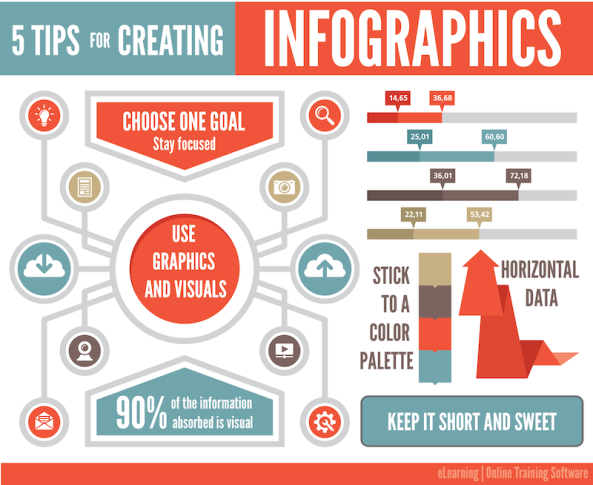
\includegraphics[width=0.8\paperwidth,height=0.9\paperheight]{img/creating-infographics.png}};
    \tikz [remember picture,overlay]%
    \node at (current page.north) [%
        draw={rgb,255:red,0; green,156; blue,220},
        inner sep=18pt,
        %fill={rgb,255:red,0; green,156; blue,220},
text=red,
        below=3cm,
        font=\sffamily\Huge
    ] {??END OF CHAPTER INFOGRAPHICS OR INFOBOX??};
   %%%%bottom area 
  \tikz [remember picture,overlay]%
        \shade [bottom color={rgb,255:red,0; green,156; blue,220},top color=white]($(current page.south west)!0!(current page.north west)$) rectangle  ($(current page.south east)!0.1!(current page.north east)$);
% \tikz [remember picture,overlay]%
%    \draw [draw={rgb,255:red,0; green,156; blue,220}, fill={rgb,255:red,0; green,156; blue,220}]($(current page.south west)!0!(current page.north west)$) rectangle  ($(current page.south east)!0.1!(current page.north east)$);
 
  \tikz [remember picture,overlay]%
    \node at (current page.south) [%
        draw={rgb,255:red,0; green,156; blue,220},
        inner sep=14pt,
        fill={rgb,255:red,0; green,156; blue,220},
        fill opacity=0.01,
        text=white,
        text opacity = 1,
        draw opacity = 0.01,
        above=0.5cm,
        font=\sffamily\Large
    ] {END OF CHAPTER};

 }

%%%%%%%%%%%%%%%%%%%%%%%%%%%%%%%%%%%
%Book end page 
\usetikzlibrary{calc,positioning}% [0]
\def\BookEndPage{%
 %%%%shaded area
  \tikz [remember picture,overlay]%
        \shade [bottom color={rgb,255:red,0; green,156; blue,220},top color=white]($(current page.south west)!0!(current page.north west)$) rectangle  ($(current page.south east)!1!(current page.north east)$);

%\tikz [remember picture,overlay]%
%    \node [anchor=south west] (titlepic) at ($(current page.south west)!0.2!(current page.north west)$){\resizebox{\paperwidth}{!}{\usebox{\titlepagepic}}};

 %%%%logo 
  \tikz [remember picture,overlay]%
    \node [anchor=south west] (logo) at (-1cm, -21.5cm) {\resizebox{!}{2cm}{\usebox{\unidologowhite}}};
   %%%%bottom area text
  \tikz [remember picture,overlay]%
    \node [anchor=south west] (text) at (0.9cm, -23.2cm) [%
        draw={rgb,255:red,0; green,156; blue,220},
        inner sep=14pt,
        fill={rgb,255:red,0; green,156; blue,220},
        fill opacity=0.01,
        text=white,
        text opacity = 1,
        draw opacity = 0.01,
        %below=4cm,
        %right=2cm,
        font=\sffamily
    ] {\begin{tabular}{l}
    Vienna International Centre · P.O. Box 300 · 1400 Vienna · Austria  \\ 
    Tel.: (+43-1) 26026-o · E-mail: info@unido.org\\
    www.unido.org
\end{tabular}};
 }
%%%%%%%%%%%%%%%%%%%%%%%%%%%%%%%%%%%
%% Hyphenation of stuborn words
\hyphenation{INDSTAT}

\hyphenation{acad-e-my acad-e-mies af-ter-thought anom-aly anom-alies
an-ti-deriv-a-tive an-tin-o-my an-tin-o-mies apoth-e-o-ses
apoth-e-o-sis ap-pen-dix ar-che-typ-al as-sign-a-ble as-sist-ant-ship
as-ymp-tot-ic asyn-chro-nous at-trib-uted at-trib-ut-able bank-rupt
bank-rupt-cy bi-dif-fer-en-tial blue-print busier busiest
cat-a-stroph-ic cat-a-stroph-i-cally co-authoring con-gress cross-hatched data-base
de-fin-i-tive de-riv-a-tive dis-trib-ute dri-ver dri-vers eco-nom-ics
econ-o-mist elit-ist equi-vari-ant ex-quis-ite ex-tra-or-di-nary
flow-chart for-mi-da-ble forth-right friv-o-lous ge-o-des-ic
ge-o-det-ic geo-met-ric griev-ance griev-ous griev-ous-ly
hexa-dec-i-mal ho-lo-no-my ho-mo-thetic ideals idio-syn-crasy
in-fin-ite-ly in-fin-i-tes-i-mal ir-rev-o-ca-ble key-stroke
lam-en-ta-ble light-weight mal-a-prop-ism man-u-script mar-gin-al
meta-bol-ic me-tab-o-lism meta-lan-guage me-trop-o-lis
met-ro-pol-i-tan mi-nut-est mol-e-cule mono-chrome mono-pole
mo-nop-oly mono-spline mo-not-o-nous mul-ti-fac-eted mul-ti-plic-able
non-euclid-ean non-iso-mor-phic non-smooth par-a-digm par-a-bol-ic
pa-rab-o-loid pa-ram-e-trize para-mount pen-ta-gon phe-nom-e-non
post-script pre-am-ble pro-ce-dur-al pro-hib-i-tive pro-hib-i-tive-ly
pseu-do-dif-fer-en-tial pseu-do-fi-nite pseu-do-nym qua-drat-ic
quad-ra-ture qua-si-smooth qua-si-sta-tion-ary qua-si-tri-an-gu-lar
quin-tes-sence quin-tes-sen-tial re-arrange-ment rec-tan-gle
ret-ri-bu-tion retro-fit retro-fit-ted right-eous right-eous-ness
ro-bot ro-bot-ics sched-ul-ing se-mes-ter semi-def-i-nite
semi-ho-mo-thet-ic set-up se-vere-ly side-step sov-er-eign spe-cious
spher-oid spher-oid-al star-tling star-tling-ly sta-tis-tics
sto-chas-tic straight-est strange-ness strat-a-gem strong-hold
sum-ma-ble symp-to-matic syn-chro-nous topo-graph-i-cal tra-vers-a-ble
tra-ver-sal tra-ver-sals treach-ery turn-around un-at-tached
un-err-ing-ly white-space wide-spread wing-spread wretch-ed
wretch-ed-ly Eng-lish Euler-ian Feb-ru-ary Gauss-ian
Hamil-ton-ian Her-mit-ian Jan-u-ary Japan-ese Kor-te-weg
Le-gendre Mar-kov-ian Noe-ther-ian No-vem-ber Rie-mann-ian Sep-tem-ber}